\section{Exchange Transactions}
\label{section:exchange_transactions}

% \subsection{Markets}

% One effort to explain the sustained failure or markets to equilibriate at the aggregate level is to
% try to explain failure of equilibriation as a result of the way individual economic behaviour
% aggregates to failure or otherwise of markets for single products to equilibriate, and further to
% explain failure of markets to equilibriate at the aggregate level.
% 
% A fundamental method of science and engineering is to assume as a first step, is to use the mean
% value to aggregate a collection of micro-level behaviours. Often this turns out not to be correct,
% but invariably, in virtually every system we seek to explain, there are some parts of the system we
% explain away by averaging out noisy behaviour. 
% 
% If we use the same technique for understanding economic behaviour, we would, as a first step assume
% that we can average markets for single goods or services, result in an aggregate supply or demand
% close to zero.
% 
% If we use the same technique for understanding economic behaviour, we would, as a first step assume
% that we can aggregate our model of supply and demand for single goods or services, and arrive at a
% aggregate where aggregate supply or demand is close to zero.
% 
% Since this conclusion is contrary to facts, economists have directed their efforts at modifying the
% supply and demand model in many ways in an effort to explain this contradiction between fact and
% theory.
% 
% What is clear, however, is that the explanation has to be sufficiently fundamental to explain the
% remarkably consistent fact of excess aggregate supply and the rarity of aggregate market
% equilibrium. As put forward by Lucas, economists have yet to find a convincing understanding of
% this fact, let alone to find a solution to the problem of equilibrium failure or the problem of
% a sustained positive unemployment rate. 
% 
% Since our explanation of these facts is outside is not a part of the supply and demand model, we
% assume our simplest model of market behaviour, and that markets at the aggregate level do in fact
% equilibriate, relying on the law of large averages.

\subsection{An Exchange Transaction Only Model}

We will start with a model simplified from Figure \ref{fig:economic_feedback_schema1}. that includes only
exchange transactions.

\begin{figure}[H]
\centering
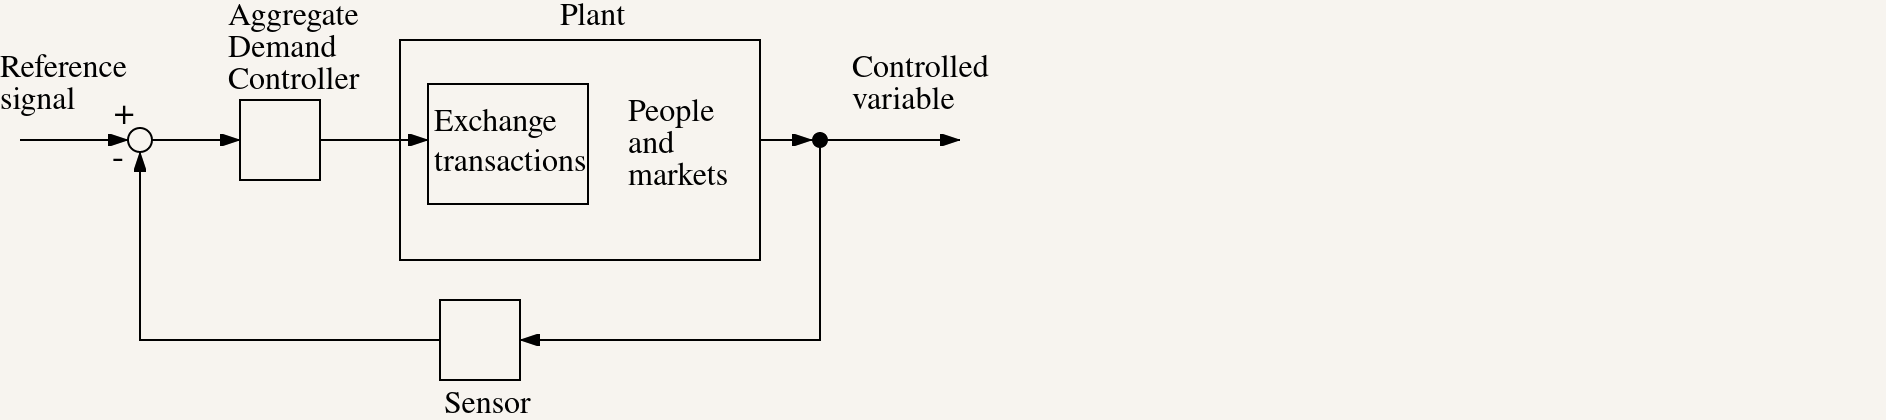
\includegraphics[scale=0.60]{03_exchange_transactions/png/exchange_only_feedback_schema}
\caption{Exchange Only Feedback Schema}
\label{fig:exchange_only_feedback_schema1}
\end{figure}

\subsection{Price and Quantity}

An exchange transactions can be characterized by a payment. We will use the unit ``dollar''
for payments. In exchange for a payments is a quantity of goods or services of a certain goods
category. We denote the quantity with a unit specific to the goods category. The price of the
transaction is the ratio of payment to quantity and the unit is dollars per unit of the goods
category. These variables relate directly to properties of transactions which indicate the state
change in a set of accounts. They are precise and measurable quantities, so we treat them
differently to measures of economic measures which try to handle some notion of human good. We
denote $f_i$ are the sum of payments for a given goods category $i$ over a period of time The unit
for any $i$ is ``dollars''. We denote the quantity of that goods category transacted in
exchange for these payments $q_i$. The unit can be different for each $i$. The average price of each
goods category is 

\[
    p_i = \frac {f_i} {q_i}
\]

We can sum $f_i$ for all transactions in a given period.

\begin{equation}\label{equation:f}
    F = \sum_i f_i
\end{equation}

As will be shown later, the aggregate value we are interested in is an accurate measure of the price
level such that a person own $x$ dollars now has the same purchasing power at any time in the
future. To make this more precise we need to define purchasing power. 

Suppose we have an economy at time $t=0$ that makes transactions 

\[
    \left( q_1, \dots, q_n \right)
\]

where there are $n$ goods categories, and the unit of quantity for each goods category may be
different. We write the units corresponding to each goods category as

\[
    \left( \left[ q_1 \right], \dots, \left[ q_n \right] \right)
\]

The average price for all transactions within a good category can be written

\[ 
    \left( p_1, \dots, p_n \right)
\]

with the corresponding units

\[
    \left( \frac {\$} {\left[ q_1 \right]}, \dots, \frac {\$} {\left[ q_n \right]} \right)
\]






We need to specify this more precisely. The quantity and proportion of different goods
transacted using a currency changes over time. We use the notion of purchasing power to construct a
measure to handle this. We can image an ``abstract person'' who we feed dollars, and make random
selections of goods and services \textit{per dollar}.  So we want to find numbers $P$ and $P'$ such
that the following
equation holds

\begin{equation}\label{equation:p_requirement}
    \frac 1 P \left[ \frac {p_1 q_1} F + \cdots + \frac {p_n q_n} F \right]
    = \frac 1 {P'} \left[ \frac {p_1' q_1'} {F'} + \cdots + \frac {p_n' q_n'} {F'} \right]
\end{equation}

Variables without a dash refer to time period $t=0$ while variables with a dash refer to time period
$t=1$. This is a dynamic equation, i.e. it defines relations relations across time. We'll proceed by
constructing some measures of aggregate quantity and aggregate price level, and then check that
these measure do conform to our requirement in equation (\ref{equation:p_requirement}). First, we
want to construct a measure of price level $P$ as a function of $p_1, \dots p_n$, and a measure of
aggregate quanitity $Q$ as a function of $q_1, \dots q_n$. These are static variables, dependent
only on other variables that are measured at the same time. But the problem is that we can't
aggregate some $Q$ from $q_1, \dots q_n$ because the units for each goods category can be different.
This also means we can't aggregate some $P$ from $p_q, \dots q_n$ because the units for $p_i$ are

\[
    \left[ \frac {\$} {i} \right]  
\]

where $i$, the units the goods category is measured in, can be different. The way we get around this
problem is to constrain the units we are working in. As an aside, it is interesting to note that
David Hume's argument heavily relies on the price units.  What we are doing here is extending Hume's
notion to both price units and quantity units. 

If at any period of time the following quantities of goods are transacted

\[
    \overline Q = \left( q_1, \dots ,q_n \right)
\]

then we choose any set of units $ \dot Q = c \overline Q $. In other words we choose a ``basket of
goods'' that is an exact multiple of the actual goods transacted at any time. This quantity has the
units

\begin{equation}\label{equation:basket}
    \left[ B \right] = \left( \left[ c q_1 \right] \dots \left[ c q_n \right] \right)
\end{equation}

and now we define $P$ as the quantity of baskets $B$ that make up total transactions $F$, i.e.  

\[
    F = P Q
\]

The units of $P$ are $\left[ \frac {\$} B \right]$. Very much like $f_i$ is independent of the
scalar value of a goods category unit we choose, $F$ in independent of the scalar value of the
basket of goods we choose, given that equation (\ref{equation:basket}) holds. We now look at the
dynamics. We have one degree of freedom remaining, i.e. our choice of $c$. At any time period, we
can choose an arbitrary $c$ but our goal is to be able to compare aggregate price across time. The
problem we face is that the relative proportions and prices $p_i$ and $q_i$ can change across time.

The problem becomes trivial if the proportions do not change, we just use the same unit for all time
periods. To account for changes in relative proportions of prices and quantities, which directly map
into changes in our basket of goods, we need to relative change in the makeup of the basket of goods
from aggregate changes. We do this by taking setting $c$ and $c'$ such that the average change in
quantities of goods in our basket remain constant, weighted by relative proportion of spending
$ \frac {f_i} F $.

\begin{equation}
    \frac {c'} c = \frac {\varepsilon [ B ]} {\varepsilon [B']}
\end{equation}

where the expected value $\varepsilon$ is weighted by $\frac {f_i} F$. This can be written

\[
    \frac 1 c \left[ \frac {f_1} F q_1 + \dots + \frac {f_n} F q_n \right] =
    \frac 1 {c'} \left[ \frac {f_1'} {F'} q_1' + \dots + \frac {f_n} {F'} q_n' \right]
\]

Increasing $c$ by a factor, reduces $Q$ by this factor, and increases $P$ by this factor.

\subsection{Concrete Example}

To make this clearer, lets look at a concrete example. Lets say there are two goods (maybe apples
and bananas) are transacted in a digital currency $a$ and $b$.

In the first period the transactions are

    \begin{twocol}
        2 apples  & \$2 \\
        4 bananas & \$1 \\
    \end{twocol}

and in the second period the transactions are

    \begin{twocol}
        3 apples  & \$2 \\
        4 bananas & \$1 \\
    \end{twocol}

In the first time period we construct a basket with units $\left[ 0.5(2 \textrm{apples}, 4
\textrm{bananas}) \right]$.

% $F=8$, $Q=2$, and $P=4$. 

% In the second time period we construct a basket with units $left[0.25(0.75 \textrm{apples},  

\subsection{Control of Price Level}

Before examining exchange transactions, we will briefly consider the feedback control mechanism.
Indexation is an important method for controlling distributed systems like a currency. An index is a
single value that is utilized by multiple components. An example of indexation in digital currencies
is Bitcoin's method for regulating the rate of production of blocks by Bitcoin miners. In this case
the indexation is algorithmic rather than controlled by a central authority. TODO

Another example of indexation is 

The simplest way to control the price level in a digital currency is to use indexation.





TODO

The feedback control loop does not work, however, in legacy currencies because the core currency
doesn't account for all money. Most money in legacy currencies is banking money, termed M1, M2 and
M3. Under these conditions, money authorities must use alternative methods to try and induce
financial institutions to increase the amount of banking money mainly through changing the interest
rate at which the money authority lends core currency to those financial institutions. At times this
method has been effective at controlling the price level, at other times less so. The process lacks
precision and has a long time-lag, making its use as the main mechanism for controlling economic
conditions problematic. Its effectiveness is also determined by financial institution's ability and
willingness to respond to decreases or increases in the monetary authority's core lending rate in a
way the maps to increases or decreases in aggregate demand.

\subsection{Market Symmetry}
